\section{Results}
\label{sec:results}

\begin{table}[t]
\centering
\caption{Main detectability and shift results. Best value per metric block is in \textbf{bold}.}
\label{tab:main-results}
\resizebox{\textwidth}{!}{%
\begin{tabular}{@{}lcccc@{}}
\toprule
Setting & AUROC & AUPRC & F1 & Accuracy \\
\midrule
Chance baseline & 0.5000 & 0.5000 & 0.5000 & 0.5000 \\
Primary holdout (seed 42) & \textbf{0.8827} & \textbf{0.9032} & 0.7750 & 0.7500 \\
Robustness eval (seed 7) & \textbf{0.9103} & -- & \textbf{0.8527} & \textbf{0.8417} \\
\midrule
Statistic & \multicolumn{4}{c}{Value} \\
\cmidrule(lr){1-5}
AUROC permutation $p$-value & \multicolumn{4}{c}{$9.99\times 10^{-4}$} \\
AUROC bootstrap 95\% CI & \multicolumn{4}{c}{[0.798, 0.952]} \\
MMD statistic & \multicolumn{4}{c}{0.02246} \\
MMD permutation $p$-value & \multicolumn{4}{c}{0.001996} \\
\bottomrule
\end{tabular}%
}
\end{table}


\para{Main finding: output-only detectability is strong.}
On held-out questions, \tfidflogreg reaches AUROC 0.8827 and AUPRC 0.9032. Accuracy is 0.75 and F1 is 0.775. The AUROC permutation test rejects chance ($p=9.99\times10^{-4}$), and bootstrap uncertainty remains well above random (95\% CI $[0.798, 0.952]$).

\para{Distribution shift is statistically significant.}
Feature-space two-sample testing reports \mmd$=0.02246$ with permutation $p=0.001996$, rejecting equal-distribution null hypotheses. This aligns with the classifier evidence and supports the central claim that lie instructions alter output distributions.

\para{Robustness under seed shift.}
When evaluated on seed-7 outputs (unseen decoding seed), AUROC increases to 0.9103 with F1 0.8527 and accuracy 0.8417, suggesting that the detector is not tied to one random draw.

\begin{table}[t]
\centering
\caption{Selected stylometric feature shifts (truthful vs.
lie-roleplay, seed 42). We report two-sided test statistics with BH-FDR correction.}
\label{tab:feature-shift}
\begin{tabular}{@{}lcccc@{}}
\toprule
Feature & Truthful mean & Lie mean & Cohen's $d$ & FDR-corrected $p$ \\
\midrule
\texttt{punct\_ratio} & 0.0383 & 0.0236 & 0.83 & $1.97\times10^{-13}$ \\
\texttt{n\_words} & 41.43 & 45.05 & -0.20 & 0.2190 \\
\texttt{upper\_ratio} & 0.0307 & 0.0243 & 0.26 & 0.0998 \\
\texttt{certainty\_ratio} & 0.0010 & 0.0019 & -0.16 & 0.1652 \\
\bottomrule
\end{tabular}
\end{table}


\para{Feature-level analysis and error profile.}
One univariate marker stands out: \texttt{punct\_ratio} drops under lie conditioning and remains significant after FDR correction. Still, most single features are weaker, indicating that separability is distributed across lexical/stylometric dimensions. On the primary holdout, the confusion matrix is TN=23, FP=13, FN=5, TP=31. False negatives are less frequent than false positives, which is favorable for safety monitoring but indicates calibration trade-offs.

\begin{figure}[t]
    \centering
    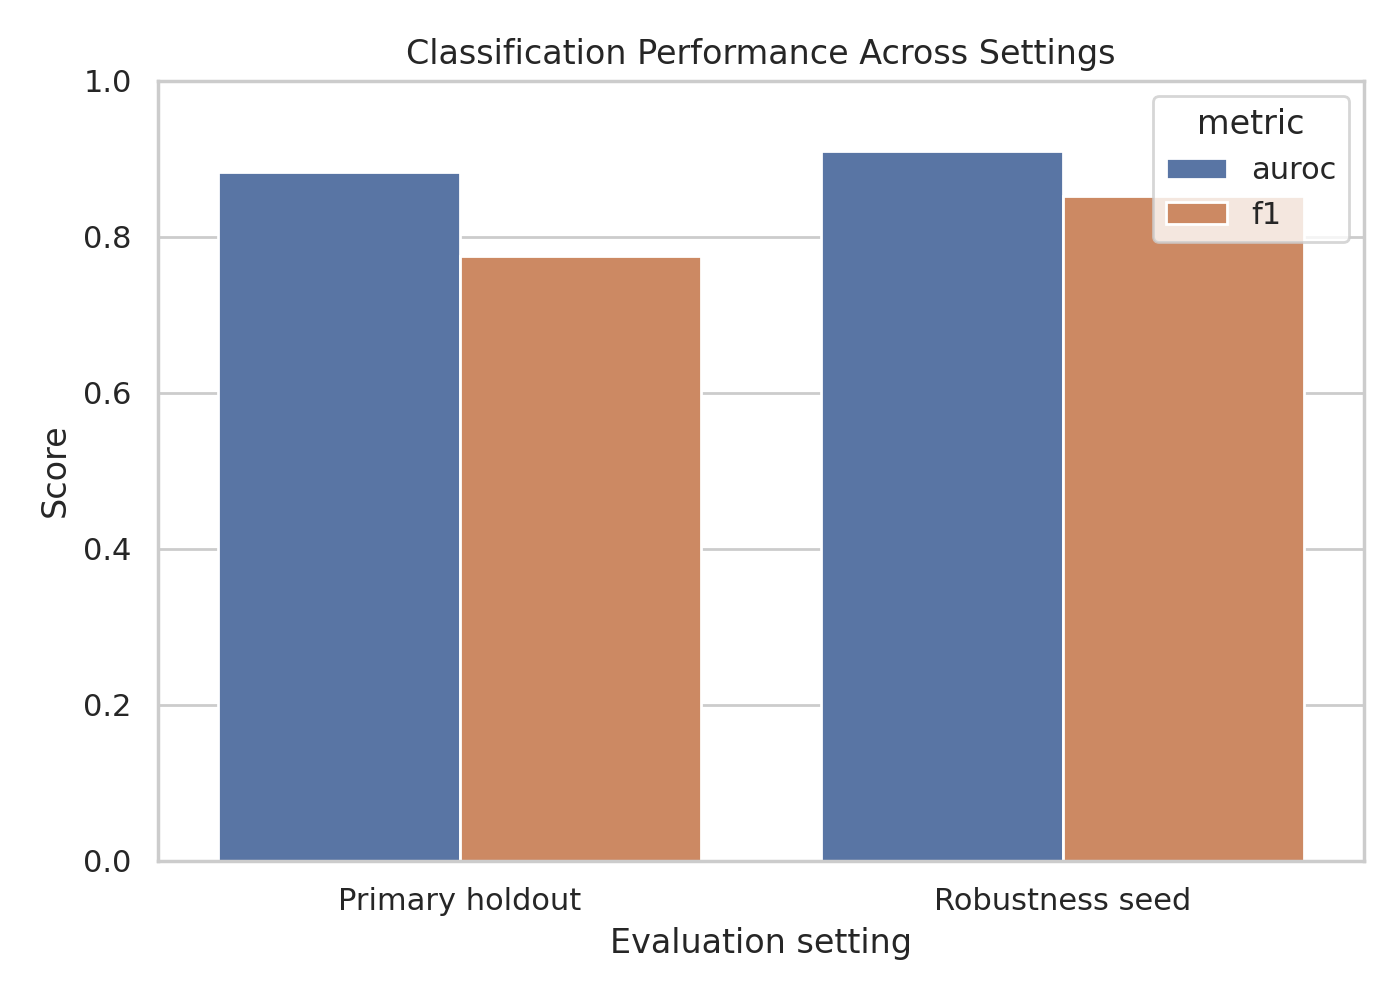
\includegraphics[width=0.95\linewidth]{figures/classification_performance.png}
    \caption{Classification summary for truthful vs.
lie-roleplay outputs. The model achieves strong AUROC/AUPRC and stable thresholded performance.}
    \label{fig:clf}
\end{figure}

\begin{figure}[t]
    \centering
    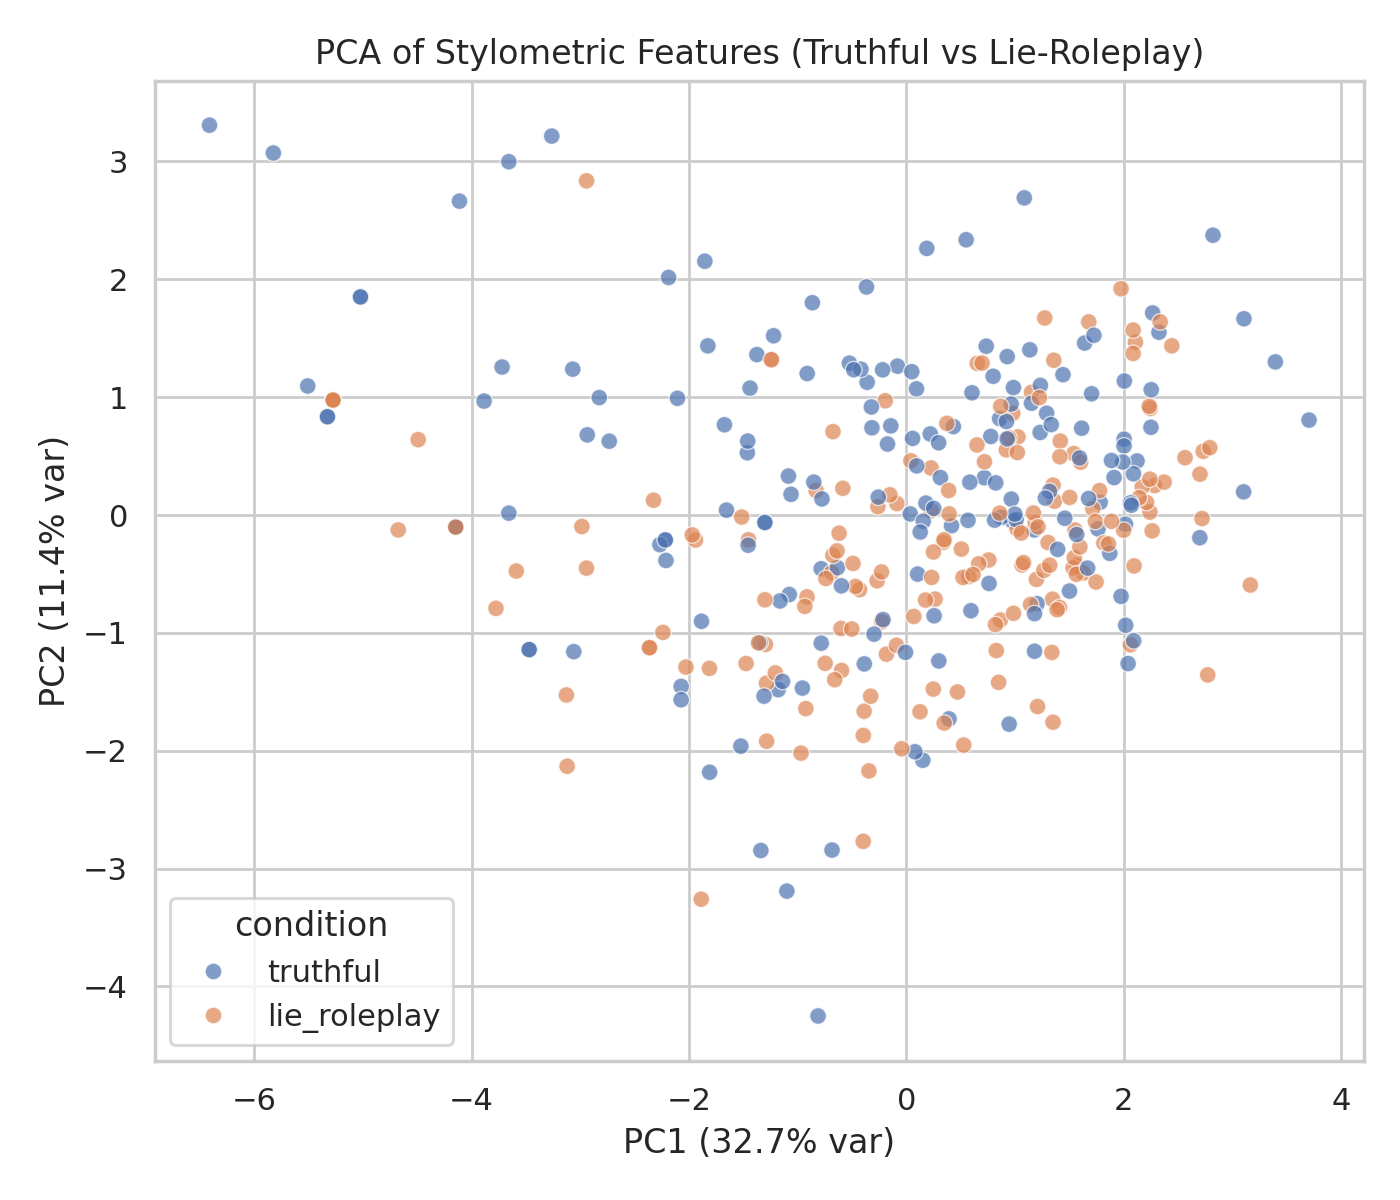
\includegraphics[width=0.95\linewidth]{figures/pca_stylometry.png}
    \caption{PCA projection of stylometric feature space. Partial class separation appears even in low dimension, consistent with multivariate distribution shift.}
    \label{fig:pca}
\end{figure}

\begin{figure}[t]
    \centering
    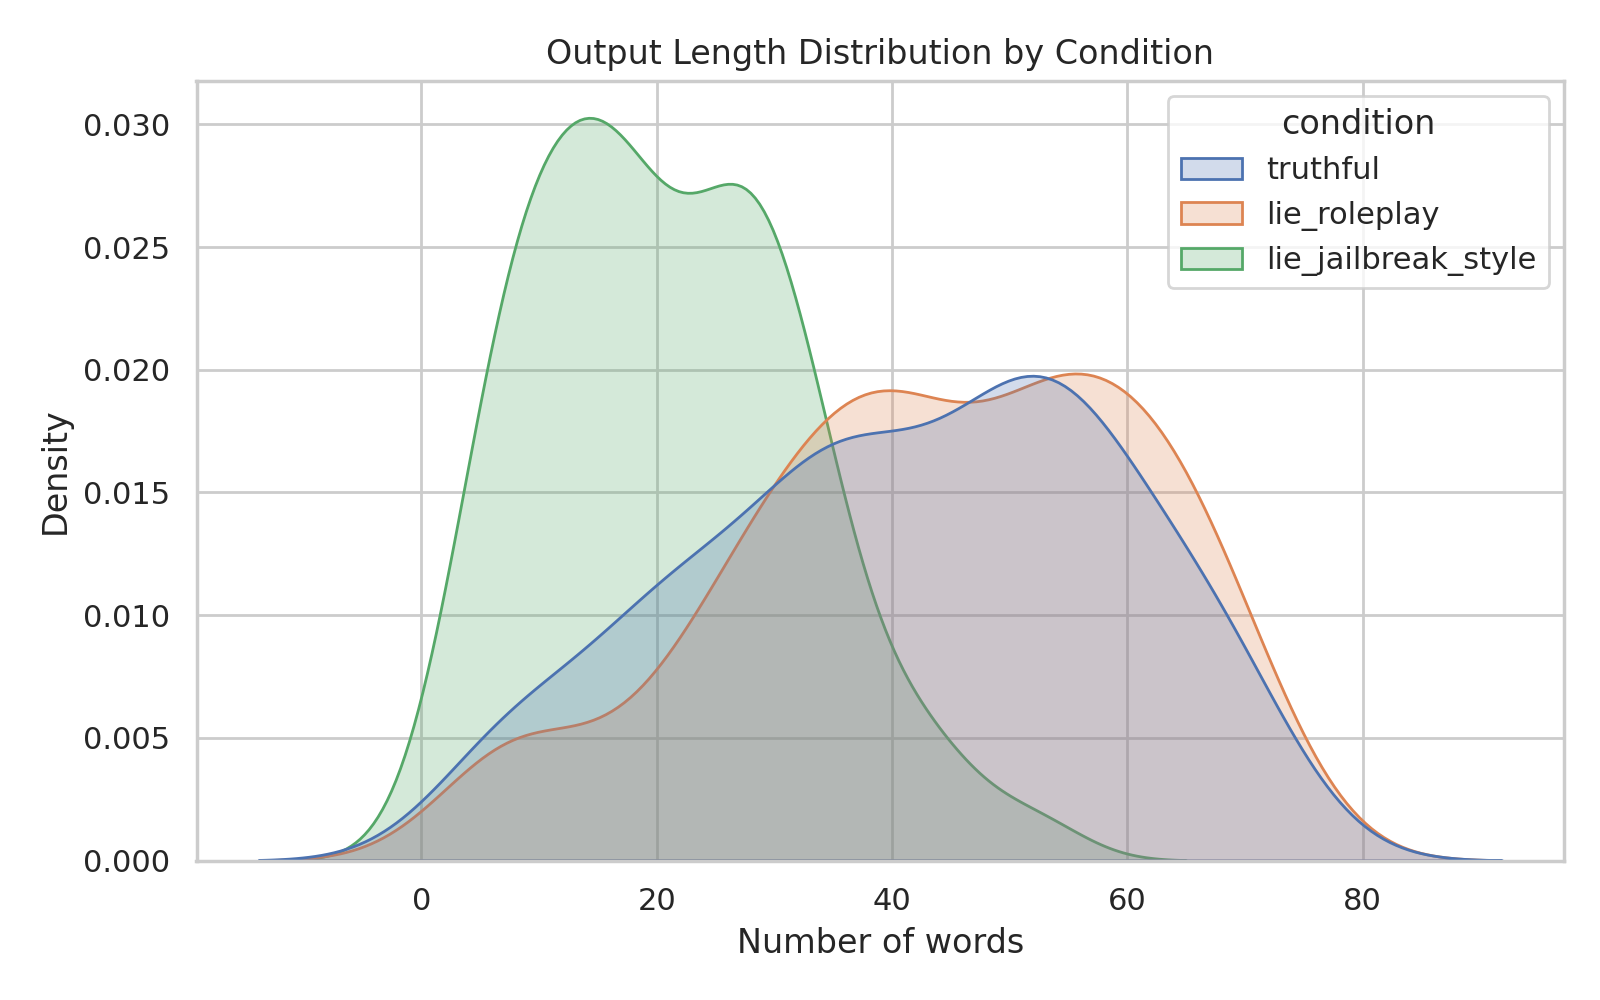
\includegraphics[width=0.95\linewidth]{figures/length_distribution.png}
    \caption{Length distributions across conditions. Length differs only modestly, indicating that detectability is not explained by verbosity alone.}
    \label{fig:length}
\end{figure}

\para{Comparison to baseline.}
Relative to random discrimination (AUROC 0.5), the observed AUROC 0.8827 yields a 76.5\% relative gain in discrimination margin.
